\chapter{Développement d'une méthode d'angiographie dynamique avec une séquence d'imagerie radiale pseudo-aléatoire par un double angle d'or ciné.}

\section{Contexte}

Afin d'apprécier la vitesse du sang dans les vaisseaux qui peut être un indicateur intéressant dans les pathologies, plusieurs méthodes sont disponibles en IRM chez l'homme. L'imagerie de prise de contraste du Gadolinium permet de visualiser l'avancée de l'agent de contraste dans les vaisseaux. Cependant, celle-ci ne permet d'obtenir que des images de basse résolution de part l'aspect d'imagerie temps réel nécessaire. De plus, malgré les avancées des méthodes d'accélération comme l'imagerie parallèle, la résolution temporelle qui peut être atteinte en imagerie 3D est supérieur à 4 secondes \cite{Grist:2012fk}.
Ces limitations ont amené l'imagerie par contraste de phase à devenir l'examen de référence pour la mesure de vitesse du sang. En effet, grâce à l'application d'un gradient bipolaire de durée et d'intensité déterminés, le déphasage des spins est alors proportionnelle à la vitesse du flux. Cette méthode a pour principal avantage d'offrir une visualisation de la vitesse et de la direction du flux voxel par voxel. Toutefois, les temps d'acquisitions sont important avec ces séquences puisqu'il est nécessaire de répéter les répéter 4 fois pour encoder la vitesse dans toutes les directions en imagerie 3D \cite{Wu:2013ys,Robson:2010uq,Johnson:2010uq}.
Il existe d'autres méthodes permettant d'estimer la vitesse des flux grâce à des acquisitions multiples avec ou sans marquage des spins sanguins puis une soustraction des images obtenues \cite{Koktzoglou:2009fe}.
Une méthode basé sur l'imagerie ciné temps-de-vol (Time-Of-Flight : TOF) a été développée au sein du laboratoire \cite{Miraux:2006fu}. Celle-ci consiste, après la détection d'un pic ECG, à saturer le signal dans le volume puis à recueillir le signal du sang frais progressant dans les vaisseaux \ref{fig:SeqSylvain}. 

\begin{figure}[H]
\centering
\line(1,0){400} \\
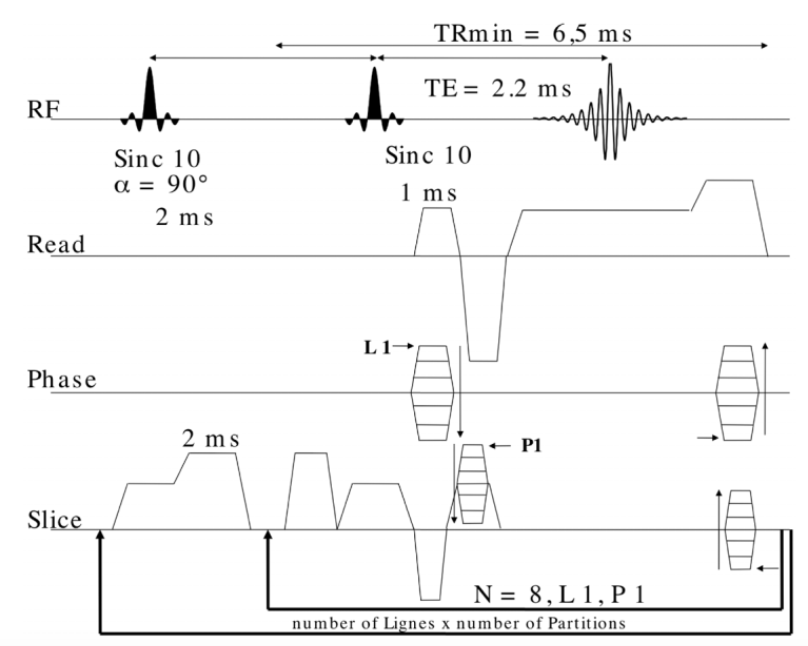
\includegraphics[scale=0.5]{./figure/chap3/SeqSylvain.png}
\caption[Séquence ARM Sylvain et al.]{\label{fig:SeqSylvain} Chronogramme de la séquence utilisé pour obtenir une ARM sang-blanc résolue dans le temps. L = Nombre de ligne, P = Nombre de partition, N = Nombre d'images résolues dans le temps reconstruites. (Figure extraite de Sylvain et al. 2006)}
\line(1,0){400} \\ \end{figure}

Les problématiques que l'on peut rencontrer chez le petit animal ne sont pas les mêmes que chez l'humain ce qui limite l'utilisation de certaines séquences ou nécessite une adaptation. L'une des limitations principales pour effectuer la mesure de flux chez la souris est son rythme cardiaque supérieur à 400 battements par minutes. La résolution temporelle de la séquence doit dont être importante pour obtenir une bonne visualisation de la dynamique des flux.
La méthode d'imagerie de flux par temps-de-vol a permis de mesurer les flux sanguin dans diverses artères chez la souris : carotides \cite{Miraux:2006fu}, pulmonaires \cite{Cochet:2013dk} et même coronaires \cite{Cochet:2010ec} ainsi que dans le polygone de Willis.

Néanmoins, le temps d'acquisition pour cette angiographie ciné 3D reste long, en particulier lorsqu'il est nécessaire d'obtenir des images avec des résolutions spatiales et temporelle élevées. Pour réduire ces temps d'acquisitions, les techniques d'imagerie parallèle peuvent être utilisé mais avec le matériel disponible en imagerie pré-clinique un gain maximum d'un facteur 2 peut être atteint et au détriment du rapport S/B. C'est pourquoi, j'ai choisi de m'orienter vers les techniques d'acquisitions radiale parce qu'elles permettent en théorie d'obtenir de fort facteur de sous-échantillonnage.

L'idée que je développerai dans ce chapitre est de combiner la méthode d'angiographie dynamique par temps-de-vol avec des trajectoires 3D radiales plutôt que cartésiennes. De plus, nous avons implémenté une méthode de répartition pseudo-aléatoire nous permettant d'obtenir une certaines flexibilité durant la reconstruction pour adapter la résolution temporelle selon la qualité des images désirées.

\section{Angiographie à partir de séquence radiale.}

L'un des inconvénient de la trajectoire cartésienne est son manque de flexibilité dans la reconstruction de l'image. Une fois que la résolution temporelle a été déterminé par le nombre de ligne successives à recueillir pour chaque répétition, il est difficile d'obtenir des images de bonne qualité (à partir du même jeu de donnée) avec une résolution temporelle différente.
Les trajectoires radiales sont plus flexibles car elles permettent de reconstruire des images intermédiaires sans attendre d'avoir recueillis toutes les projections de l'espace de Fourier. Mais, comme montré dans la figure \ref{fig:SousEchant}, cela est très dépendant de la méthode de répartition des projections employées. La répartition linéaire permet d'obtenir une répartition homogène des projections lorsque toutes les données sont recueillies mais elle manque de flexibilité lors de la reconstruction d'une image n'utilisant seulement qu'une partie des données recueillies durant un temps donné. Il est donc nécessaire de proposer des répartitions pseudo-aléatoires qui permettront de répartir de manière plus homogène les projections au cours du temps et donc d'obtenir des images de meilleur qualité par example dans la figure {fig:SousEchan}.droite.

\begin{figure}[H]
\centering
\line(1,0){400} \\
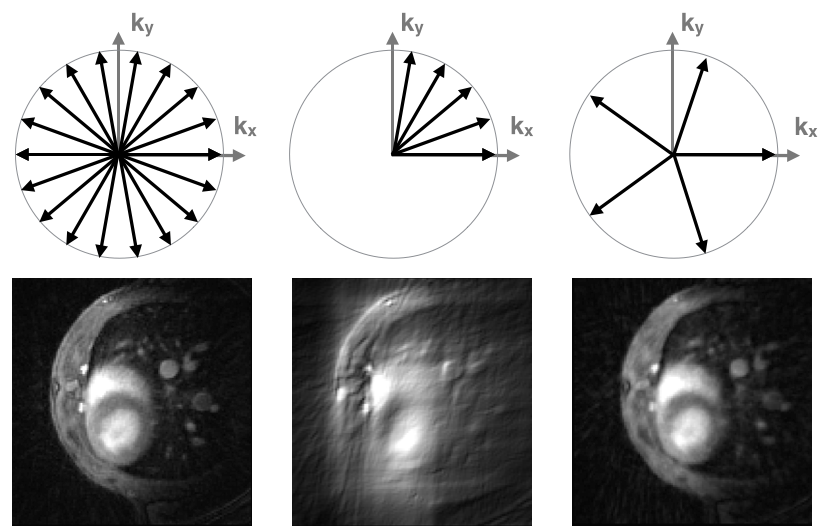
\includegraphics[scale=0.5]{./figure/chap3/SousEchan.png}
\caption[Sous-échantillonnage]{\label{fig:SousEchan} Vue axiale obtenue avec une séquence UTE 2D sur le coeur de souris. A gauche : l'image est reconstruite avec les 402 projections pour atteindre le critère de Nyquist. Au centre : l'image est acquises avec 100 projections réparties de manières adjacentes par rapport au cas idéal à gauche. A droite : l'image est reconstruite avec 100 projections réparties de manière uniforme sur le plan.}
\line(1,0){400} \\ \end{figure}

De nombreuses méthodes de répartition pseudo-aléatoire des projections 2D et 3D ont été étudiées : Les méthodes utilisant des trajectoires multi-spiral \cite{Chan:2009uq}, La méthode quasirandom \cite{Tibiletti2015Multistage-thre}, les méthodes d'inversion de bit \cite{Theilmann2004View-ordering-i}, les séquences Halton \cite{chan2009halton} ou bien encore des méthodes utilisant l'angle d'or\cite{Winkelmann:2007fk}. Winkelmann et al. \cite{Winkelmann:2007fk} et Song et al. \cite{Song:2000fk} ont montré que l'imagerie radiale 2D est plus flexible en utilisant un angle d'or, dérivé du facteur d'or (décris dans la prochaine section). Par example en imagerie de prise de contraste dynamique, en positionnant les projections dans l'espace de Fourier avec cet angle, il est possible à partir de n'importe quelle position de reconstruire une image. Le nombre de projection a utiliser peut-être adapté pour modifier à la résolution spatiotemporelle. Chan et al. \cite{Chan:2009uq} ont montré qu'il était possible d'étendre la notion d'angle d'or à l'imagerie radiale 3D et ont montré son application à l'imagerie dynamique de prise de contraste dans les tumeurs du sein.

J'ai décidé de m'orienter vers l'utilisation de cette méthode qui a montré une meilleur flexibilité par rapport aux méthodes d'inversion de bit, halton et de multi-spiral dans les conditions de fort sous-échantillonnages recherchées.

\subsection{Angle d'or}

L'angle d'or $\phi$ est dérive du facteur d'or qui est extrait de la suite de Fibonacci. Il est utilisé en IRM pour de nombreuses applications permettant de répartir au mieux des données dans l'espace de Fourier, que ce soit en imagerie cartésienne \cite{derbyshire2011golden} ou radiale. En imagerie radiale projection-reconstruction celui-ci est égale à $\phi=111,24 \degres$. Chaque projection est donc séparé par cet angle de la précédente. Cela a pour effet de bien répartir spatialement et temporellement les projections au cours du temps.

\begin{figure}[h]
\centering \line(1,0){400} \\
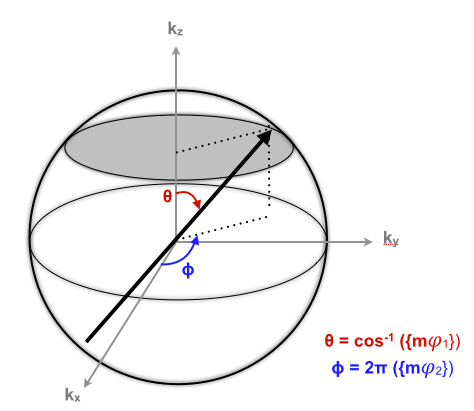
\includegraphics[scale=0.4]{./figure/chap3/Gold3D.png}
\caption[Angle d'or 3D]{\label{fig:Gold3D} Positionnement des projections radiales dans l'espace de Fourier basé sur l'angle d'or 3D.}
\line(1,0){400} \\ \end{figure}

Ce principe d'angle d'or a été étendu à l'imagerie 3D. Deux facteurs d'or sont nécessaires à son implémentation ($\phi_1=0,4656$=,$\phi_2=0,6823$). Ici, nous utilisons une méthode de répartition des projections pour l'imagerie 3D qui utilisent $\phi_1$ pour déterminer la position selon l'axe $k_z$ et $\phi_2$ pour déterminer l'angle polaire de la projection dans le plan $k_x-k_y$ (figure \ref{fig:Gold3D}) selon les équations suivantes :
\begin{equation}
\label{eq:GoldPremier}
\begin{array}{c}
\Phi_i=2\pi \times mod(\phi_1 \times i,1) \\
\theta_i=acos(mod(\phi_2 \times i,1))
\end{array}
\end{equation}
où i est le numéro de la projection. Cette implémentation de l'angle d'or 3D ne fonctionne que pour l'imagerie projection-reconstruction car avec une trajectoire UTE un des hémisphères ne sera jamais échantillonné. Pour la trajectoire angle d'or 3D UTE, il faut modifier le calcul de $\theta$ :
\begin{equation}
\theta_i=2 \times acos(mod(\phi_2 \times i,1))-1
\end{equation}
Comme montré dans la figure \ref{fig:ComparTraj}, on observe que la répartition au cours du temps des projections est assez uniforme.


\begin{figure}[h]
\centering \line(1,0){400} \\
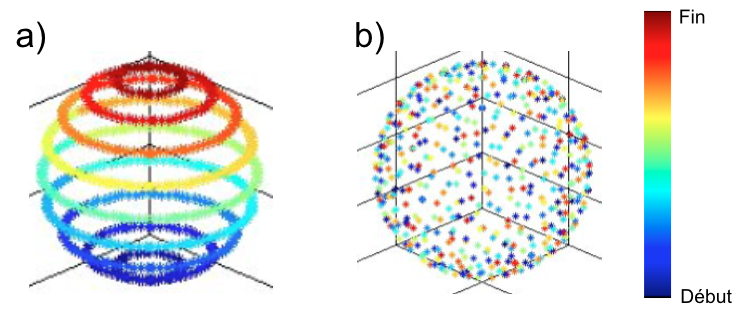
\includegraphics[scale=0.4]{./figure/chap3/ComparTraj.png}
\caption[Comparaison entre les trajectoires]{\label{fig:ComparTraj} Positionnement des derniers points de chaque projections radiales dans l'espace de Fourier basé au cours du temps grâce à la méthode : (a) utilisée sur les imageurs Bruker (b) d'angle d'or 3D (c) d'angle d'or 3D UTE.}
\line(1,0){400} \\ \end{figure}

\subsection{Angiographie anatomique avec l'angle d'or et sous-échantillonnage}

Pour vérifier les effets de l'implémentation de l'angle d'or nous avons effectué une angiographie anatomique au niveau des carotides de plusieurs souris.

La bonne qualité des images obtenues en reconstruisant un nombre décroissant de projection consécutives (40000, 8000, 4000, 2500) qui sont visible dans la figure \ref{fig:RadialAnat} est un indicateur de la bonne homogénéité de la répartition des projections avec l'angle d'or 3D.
L'effet du sous-échantillonnage se traduit par une difficulté à distinguer les parties des artères les plus faible sur les images d'intensité de projection maximum (MIP) comme indiqué par la flèche pointillée qui est provoqué par une augmentation du flou. Cependant l'angiogramme complet est bien définie avec seulement 4000 projections correspondant à un temps d'acquisition de 22 sec alors que l'on observe de nombreux artéfacts sur les images recueillies avec une séquence cartésienne malgré les temps d'acquisition 10 fois plus important. On distingue en effet la présence du repliement de la crosse aortique provoqué par un artéfact de flux sur l'image axial qui n'est pas présent sur l'image radiale. De plus le signal du sang est bien plus important et surtout plus homogène sur les images radiale en particulier aux niveaux des flux turbulent comme montré par la petit flèche blanche.

La robustesse et l'apport en SNR des séquences radiales combiné à l'utilisation de l'angle d'or 3D permet d'obtenir des images d'angiographie 3D sur le petit animal de très bonne qualité en des temps d'acquisition restreint. Ce qui est encourageant pour l'utilisation de cette trajectoire pour des séquences résolues dans le temps.

\begin{figure}[h]
\centering \line(1,0){400} \\
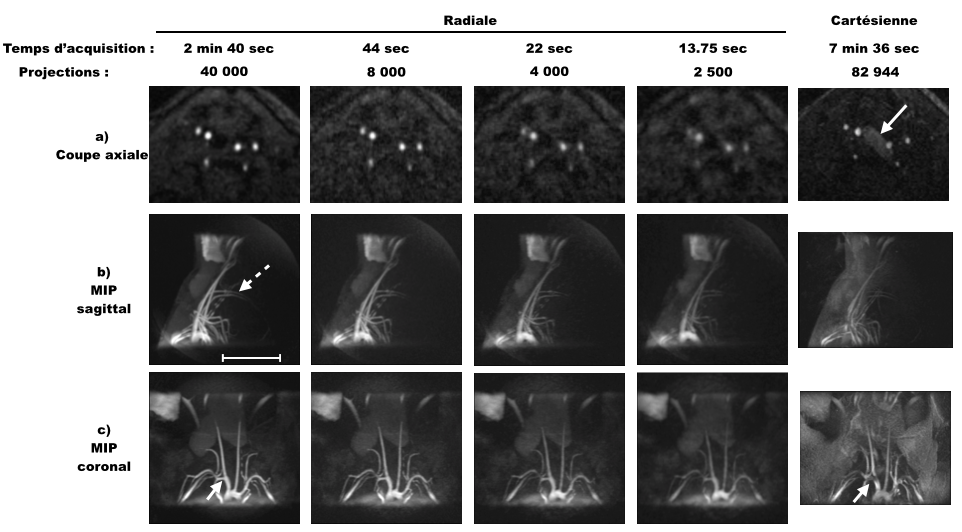
\includegraphics[scale=0.4]{./figure/chap3/RadialAnat.png}
\caption[Comparaison entre les trajectoires]{\label{fig:RadialAnat} Imagerie anatomique 3D positionnée au niveau des carotides d'une souris.}
\line(1,0){400} \\ \end{figure}

\section{Angiographie radiale résolue dans le temps.}

\subsection{Séquence}

\begin{figure}[H]
\centering \line(1,0){400} \\
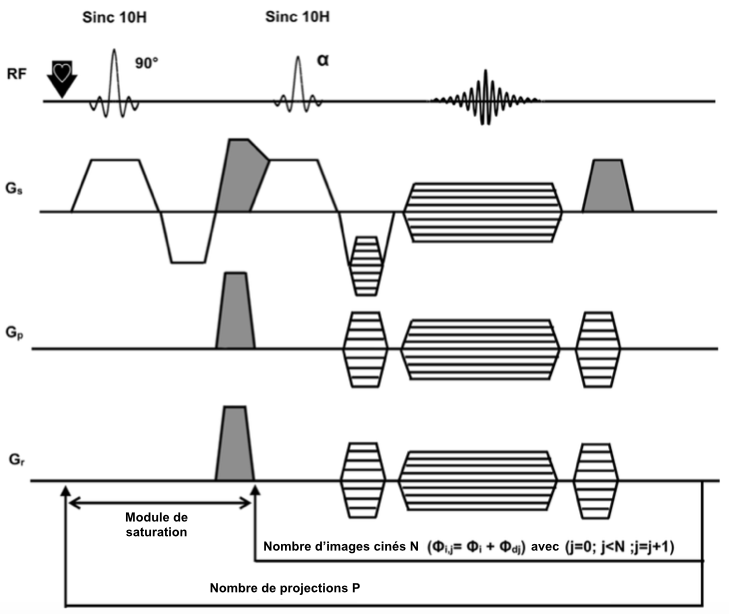
\includegraphics[scale=0.5]{./figure/chap3/SeqARMAurel.png}
\caption[Chronogramme ARM dynamique]{\label{fig:SeqARMAurel} Chronogramme de la séquence ARM sang blanc 3D radiale synchronisé sur l'ECG. Un module de saturation a été ajouté avant l'acquisition de N images cinés. Chacune de ces images a été acquises avec $P(\Phi_{i,j},\theta_i)$ projections. Pour chaque image ciné, $\Phi_{i,j} = \Phi_i+\Phi d_j$, où i est le nombre de projection et j est le nombre de ciné. Les gradients de déphasage sont indiqués en gris. La flèche noire représente la synchronisation ECG.}
\line(1,0){400} \\ \end{figure}

Le chronogramme de la séquence que j'ai développée est présentée dans la figure \ref{fig:SeqARMAurel}. Celle-ci est basée sur la méthode Miraux et al. \cite{Miraux:2006fu} et est constitué d'un module de saturation sélectif effectué sur le même volume que celui qui sera imagé. Après ce module, une séquence d'écho de gradient rapide est appliqué et est répété un nombre de fois NCiné correspondant au nombre d'images cinés que l'on souhaite reconstruire. Cette séquence d'écho de gradient est constitué d'une impulsion de radiofréquence sélective permettant d'obtenir un signal temps-de-vol dans le volume imagée. L'impulsion est suivi d'un gradient de rephasage de coupe combiné à des gradients de déphasage selon les trois axes permettant de se déplacer à l'extérieur de l'espace de Fourier. Leurs intensité est ensuite inversé pour permettre la lecture du signal selon une projection. 
L'intensité des gradients sur les axes kx, ky et kz sont modulés en fonction du numéro de la trajectoire à recueillir, ici noté i, grâce à l'équation :
\begin{equation}
\label{eq:GoldPremier}
\begin{array}{c}
kx_i = kmax \times \cos(\Phi_i) \sin(\theta_i) \\
ky_i = kmax \times \sin(\Phi_i) \sin(\theta_i) \\
kz_i = kmax \times \cos(\theta_i)
\end{array}
\end{equation}
où $\Phi_i$ et $\theta_i$ sont obtenues grâce à l'équation \ref{eq:GoldPremier} définissant les trajectoires selon l'angle d'or 3D. Des gradients de "spoiler" sont ensuite appliqué pour déphaser le signal résultant.

\subsection{Second angle d'or}

Généralement en imagerie résolue dans le temps, N signaux IRM sont recueillies successivement avec la même trajectoire dans l'espace de Fourier. Cela est répété de manière à pouvoir remplir N espaces de Fourier complets afin de pouvoir reconstruire N images (souvent appelé image ciné). Lorsque les temps de répétition sont courts par rapport aux mouvements dynamiques que l'on souhaite observer la différence entre les images est très faible et l'on obtient donc une redondance importante dans les informations contenues dans l'espace de Fourier. Or, comme expliqué dans la section \ref{subsec:KSpaceRegion}, il est possible d'exploiter les hautes fréquences pour augmenter la résolution de l'image. Cependant la méthode standard d'imagerie résolue dans le temps ne permet pas de flexibilité spatiotemporelle entre les différentes images reconstruites. Ce constat a lieu que l'on utilise des trajectoires cartésiennes ou non-cartésiennes car elle provient seulement du fait que les trajectoires utilisés entre les images cinés soient les mêmes. Pour résoudre cela, il est donc nécessaire de modifier les trajectoires entre les cinés de manière à pouvoir ensuite les manipuler par example en additionnant deux espaces de Fourier pour gagner en résolution spatiale et signal mais perdre en résolution temporelle. 

La méthode vers laquelle nous nous sommes dirigés a été de recueillir le signal de chaque cycle cardiaque avec des trajectoires similaire mais subissant seulement une rotation autour de l'axe $k_z$. L'angle que nous avons décidé d'employer $\Phi d_j$ est aussi basé sur l'angle d'or 2D $v_2$ et s'intègre dans les équations précédentes de la manière suivante :
\begin{equation}
\begin{array}{c}
\Phi_i=2\pi \times mod(\phi_1 \times i,1) +\Phi d_j\\
\theta_i=acos(mod(\phi_2 \times i,1)) \\
with \Phi d_j=2\pi \times  mod( v_2 \times j)
\end{array}
\end{equation}
où j correspond au numéro de l'espace de Fourier du cycle cardiaque qui sera complété par cette projection. Cette méthode permet donc d'obtenir une répartition des projections similaire mais avec des trajectoires d'échantillonnages de l'espace de Fourier différentes (figure \ref{fig:GoldCine}) en fonction de la position dans le cycle cardiaque. Cette méthode est plus efficace qu'une simple augmentation de la trajectoire d'un angle (360/Nombre d'images cinés) car, lors de la reconstruction, les espaces de Fourier utilisés seront les plus proches.Il est donc intéressant d'avoir un angle plus élevé qui permettra d'obtenir des trajectoires très différentes sur les cinés adjacentes plutôt que des trajectoires proches qui donneront peu de nouvelles informations pour améliorer la résolution spatiales. 
L'implémentation de ces trajectoires dans une séquence d'ARM dynamique de flux est décrite dans la figure \ref{fig:SeqARMAurel} sous forme de chronogramme.
 
\begin{figure}[H]
\centering \line(1,0){400} \\
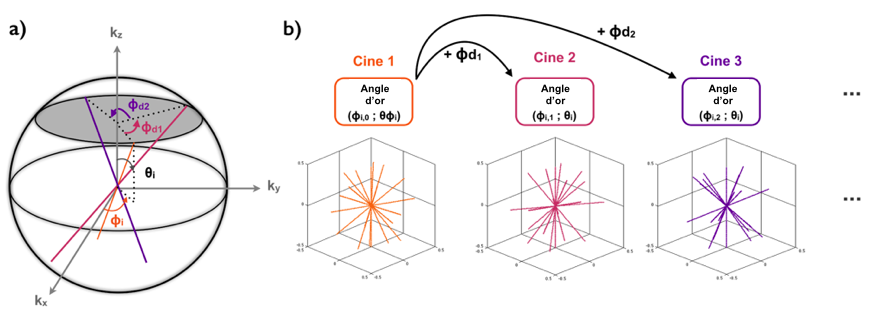
\includegraphics[scale=0.5]{./figure/chap3/GoldCine.png}
\caption[Répartition grâce à l'angle d'or entre les images ciné]{\label{fig:GoldCine} Description de la méthode utilisée pour obtenir une répartition différentes des projections entre des images cinés consécutives. (a) La ligne orange représente la trajectoire d'une projection définie par le premier angle d'or, correspondant à l'image ciné 1 . Pour l'image ciné 2 (rose), la nouvelle trajectoire est obtenue en ajoutant l'angle $\Phi d_1$. Pour l'image ciné 3 (violet), l'angle ajouté est égale à $\Phi d_2$. La même valeur d'angle $\theta_i$, est utilisé entre les projections des cinés adjacentes. (b) Exemple sur la distribution 9 projections pour 3 images cinés consécutives.}
\line(1,0){400} \\ \end{figure}

\subsection{Filtre temporel}

Pour reconstruire une image ciné à un temps donné du cycle cardiaque, nous avons utilisé un filtre temporel que nous appliquons à chaque espace de Fourier. Ce filtre temporel permet de regrouper les données de l'espace de Fourier que l'on veut reconstruire avec une partie des hautes fréquences des espaces de Fourier adjacents. De nombreux filtres différents peuvent être créés et adaptés a-posteriori lors de la reconstruction comme des filtres exponentielles ou linéaires qui s'utilisent pour des images de prises de contraste dynamique \cite{Lin:2008uq}.
Nous avons décidé d'utiliser un filtre défini par 2 paramètres, Q et R ($Q \leq R$) qui correspondent à des distances temporelles entre les espaces de Fourier dans le cycle cardiaque par rapport à l'espace de Fourier à reconstruire. Pour reconstruire l'image situé à la position x du cycle cardiaque, nous utiliserons tout l'espace de Fourier à cette position auquel nous ajouterons la moitié des hautes fréquences des espaces situé à une position s tel que : $x-Q < s \leq x+Q$ inclus. Et enfin nous ajouterons le quart des hautes fréquences des espaces de Fourier situé à une position $x-Q-R \leq s < x-Q$ et $x+Q \geq s \geq x+Q+R$. La forme de ce filtre est illustré dans la figure \ref{fig:filtre} pour des valeurs R = 3 et Q = 1.
La résolution temporelle est donc étalé sur 7 TR mais le fait de ne pas utiliser les basses fréquences dans les images cinés adjacentes permet de réduire la résolution temporelle effective.
Après application du filtre temporel on obtient un espace de Fourier que l'on peut reconstruire avec la méthode de "gridding" standard décrite dans le chapitre précédente.
L'utilisation d'un filtre temporel n'est pas uniforme sur tout le cycle cardiaque. En effet, des effets de bords réduiront la qualité des images que l'on peut obtenir au début et à la fin du cycle cardiaque.

\begin{figure}[H]
\centering \line(1,0){400} \\
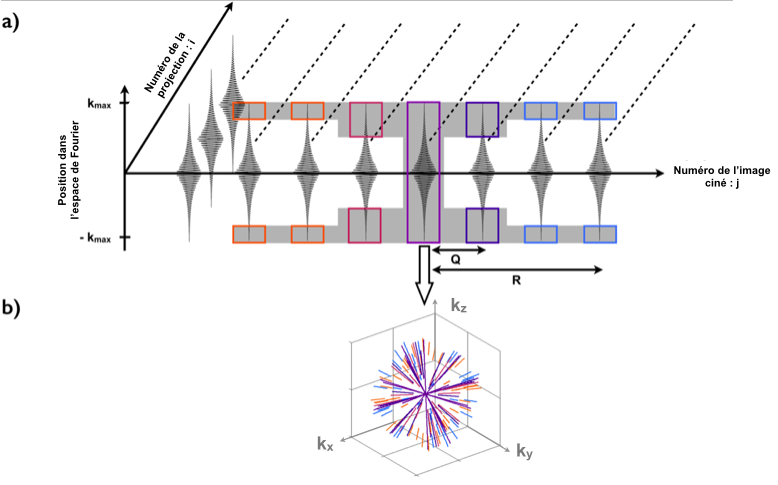
\includegraphics[scale=0.45]{./figure/chap3/filtre.png}
\caption[Filtre temporel]{\label{fig:filtre} Représentation du filtre temporel (en gris) utilisé pour reconstruire l'image ciné 5 avec Q = 1 et R = 3. (a) Les données sont reconstruites en utilisant la moitié des hautes fréquences des projections recueillies à une distance temporelle maximum Q, et un quart des projections est utilisé pour des distances temporelles plus élevées (de Q à R). (b) Représentation schématique de l'espace de Fourier de l'image ciné 5 après application du filtre temporel.}
\line(1,0){400} \\ \end{figure}

\subsection{Résultats}

Toutes les expériences décrites dans cette partie ont été effectuées sur un imageur 7T Bruker Biospec (Ettlingen, Germany) équipé avec un système de gradient capable de fournir 660 mT/m au maximum et avec un temps de monté des gradients de 110 $\mu$s.
Une antenne volumique quadratique (Diamètre interne 75.4 mm, longueur = 70 mm) est utilisée pour l'excitation et une antenne de surface à 4 éléments (dimension extérieur d'un élément d'antenne: 12 $\times$ 16 mm$ ^2$; dimension extérieure totale: 26 $\times$ 21 mm$ ^2$) est utilisée pour la réception du signal.

\subsubsection{Validation de la séquence sur fantômes}

La séquence a tout d'abord été validé sur un fantôme de flux, en particulier l'effet du sous-échantillonnage et l'utilisation du filtre temporel sur l'évaluation de la dynamique de progression des flux. Pour cela, un fantôme constitué de spins stationnaires contenu dans un cylindre remplie avec de l'eau et de spins mouvants dans un tube droit contenant de l'eau a été imagé. Le diamètre du tube est de 0,5 mm et le débit de l'eau dans le tube est de 3,75 mL/min qui correspond à une vitesse de 31,8 cm/s. La séquence n'est pas synchronisé et 20 images cinés sont recueillies. Nous avons utilisé les paramètres suivant pour l'imagerie: TE/TR = 1,5/3,3 ms; $\alpha=12\degres$; bande passante de réception = 200 kHz; FOV = 25 x 25 x 25 mm; matrice de lecture = 192; résolution spatiale = $(130 \ \mu m)^3$.
\begin{figure}[H]
\centering \line(1,0){400} \\
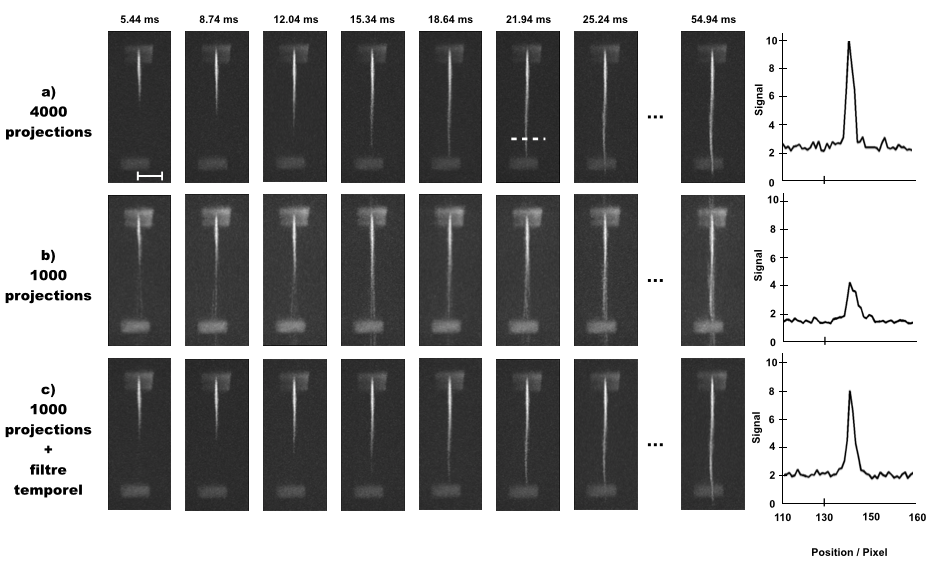
\includegraphics[scale=0.5]{./figure/chap3/ImFlowPhant.png}
\caption[Image ARM dynamique sur fantôme]{\label{fig:ImFlowPhant} Images MIP coronales recueillies sur le fantôme de flux avec la séquence dynamique. Les images reconstruites avec (a) 4000 ou (b) 1000 projections sont comparées aux images reconstruites avec (c) 1000 projections et l'utilisation d'un filtre temporel (R=3, Q=1). Le profile d'intensité est obtenu au niveau de la ligne pointillée au temps 21,94 ms pour chaque cas.}
\line(1,0){400} \\ \end{figure}

Les données sont sous-échantillonnées a-posteriori pour obtenir un jeu de donnée constitué de 1000 et 4000 projections correspondant respectivement à des temps d'acquisition de 4 min 51 s et 1 min 13 s. Avec 4000 projections (figure \ref{fig:ImFlowPhant}.a), nous arrivons a distinctement visualiser la progression du flux dans le tube et sa vitesse peut être correctement mesurée. Le pic de vitesse est égale à 65 cm/s, ce qui correspond à 2 fois la valeur moyenne. Avec 1000 projections (figure \ref{fig:ImFlowPhant}.b), on observe sur les images une nette infériorité en terme de signal et de résolution spatiale. Le signal du tube passe de 10 à 4,2 entre 4000 et 1000 projections. On observe aussi la présence d'artéfacts de streaking (flèche blanche) qui empêche la mesure d'une valeur précise de vitesse des flux. Cependant en utilisant le filtre temporel (R=3,Q=1) (figure \ref{fig:ImFlowPhant}.c) les artéfacts de streaking sont supprimés et l'on observe que le profile de signal remonte de 4.2 à 8 ce qui est environ au niveau de la reconstruction avec 4000 projections.
Nous avons mesuré l'augmentation du volume de flux dans le FOV sur toutes les images ciné (correspondant à la progression du flux dans le tube) et l'on observe une sur-évaluation du volume sur les images reconstruites avec 1000 projections. Par contre avec l'utilisation du filtre on observe des données totalement en accord avec celle reconstruite avec 4000 projections.
\begin{figure}[H]
\centering \line(1,0){400} \\
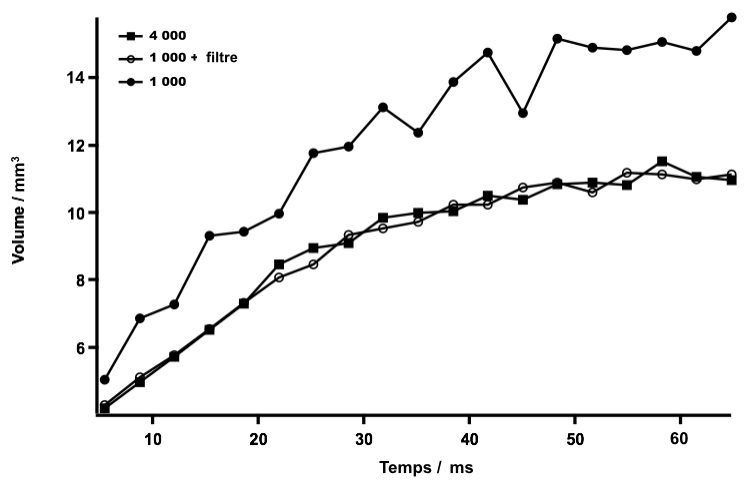
\includegraphics[scale=0.4]{./figure/chap3/GraphFlowPhant.png}
\caption[Graphique de progression du flux sur fantôme]{\label{fig:GraphFlowPhant} Volume des flux mesuré en fonction du temps après l'application du module de saturation obtenues sur fantôme. Les données représentées ont été recueillies avec 4000, 1000 et 1000 + filtre projections.}
\line(1,0){400} \\ \end{figure}

%\subsubsection{Imagerie in-vivo}
%
%Ces observations ont aussi été observé in-vivo sur les carotides de souris avec la même séquence synchronisée sur l'ECG. La comparaison des images non-filtrée et filtrée avec 1000, 2500 et 4000 projections (figure \ref{fig:ImFlowMice}) ainsi que les résultats de mesure de volume de flux (\ref{fig:GraphFlowMice}) montre qu'il est nécessaire d'utiliser un nombre de projection plus important in-vivo due à la qualité globale des images. Les images obtenue avec une reconstruction de 2500 projections et l'utilisation du filtre (R=3,Q=1) donne des résultats équivalent en terme de qualité d'image et de volume du flux. Dans la suite, nous utiliserons 2500 projections correspondant approximativement à 6 min 30 s de temps d'acquisition totale.
%\begin{figure}[H]
%\centering \line(1,0){400} \\
%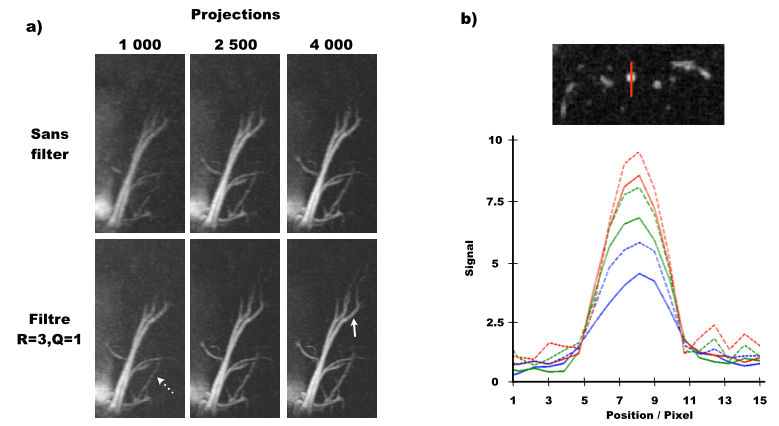
\includegraphics[scale=0.5]{./figure/chap3/ImFlowMice.png}
%\caption[Image ARM dynamique sur souris]{\label{fig:ImFlowMice} Images MIP sagital recueillies sur des carotides de souris avec la séquence dynamique. (a) Les images reconstruites avec 1000, 2500 et 4000 projections sont comparées aux images reconstruites avec l'utilisation d'un filtre temporel (R=3, Q=1). (b) Le profile d'intensité est obtenu au niveau de la ligne rouge sur les carotides après la bifurcation aortique. Lignes continues : reconstructions non-filtrées; bleu: 1000 projections; vert: 2500 projection; rouge: 4000 projections.}
%\line(1,0){400} \\ \end{figure}
%
%\begin{figure}[H]
%\centering \line(1,0){400} \\
%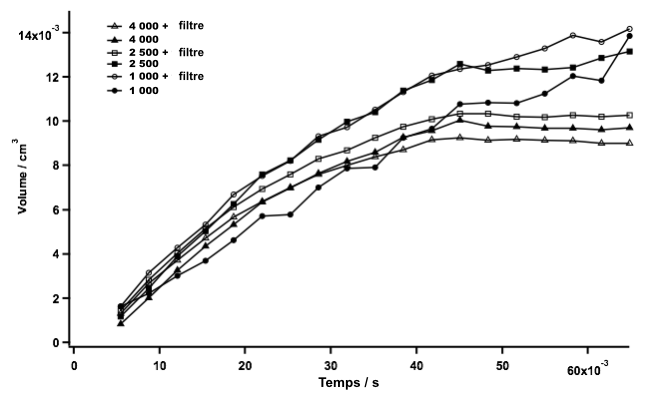
\includegraphics[scale=0.5]{./figure/chap3/GraphFlowMice.png}
%\caption[Graphique de progression du flux sur fantôme]{\label{fig:GraphFlowMice} Volume des flux mesuré en fonction du temps après l'application du module de saturation sur les carotides d'une souris saine. Les données représentées ont été recueillies avec 4000, 2500 et 1000 projections ainsi qu'avec leurs reconstruction filtrée (R=3,Q=1).}
%\line(1,0){400} \\ \end{figure}

\subsubsection{Imagerie du polygone de Willis}

\begin{figure}[H]
\centering \line(1,0){400} \\
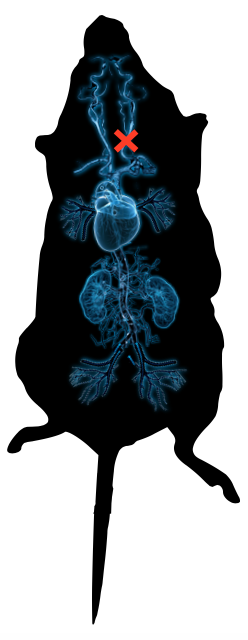
\includegraphics[scale=0.5]{./figure/chap3/LigatCarotide.png}
\caption[Modèle de ligature des carotides]{\label{fig:LigatCarotide} Schéma du modèle de ligature de la carotide sur souris}
\line(1,0){400} \\ \end{figure}

Avec la séquence d'ARM dynamique, il a été possible de visualiser chez 4 souris ayant subit une ligature de la carotide droite (figure \ref{fig:LigatCarotide}) que le remplissage du polygone était compensé par le flux sanguin provenant de la carotide droite. Cependant celui-ci arrive dans la partie droite du polygone avec un délai de retard par rapport à la souris saine (\ref{fig:ImFlowWillis}).
Ce délai a pu être quantifier sur une carte de couleur grâce à une méthode de calcule du temps d'arriver du sang en un point de l'espace (\ref{fig:ColorMapFlowWillis}).

\begin{figure}[H]
\centering \line(1,0){400} \\
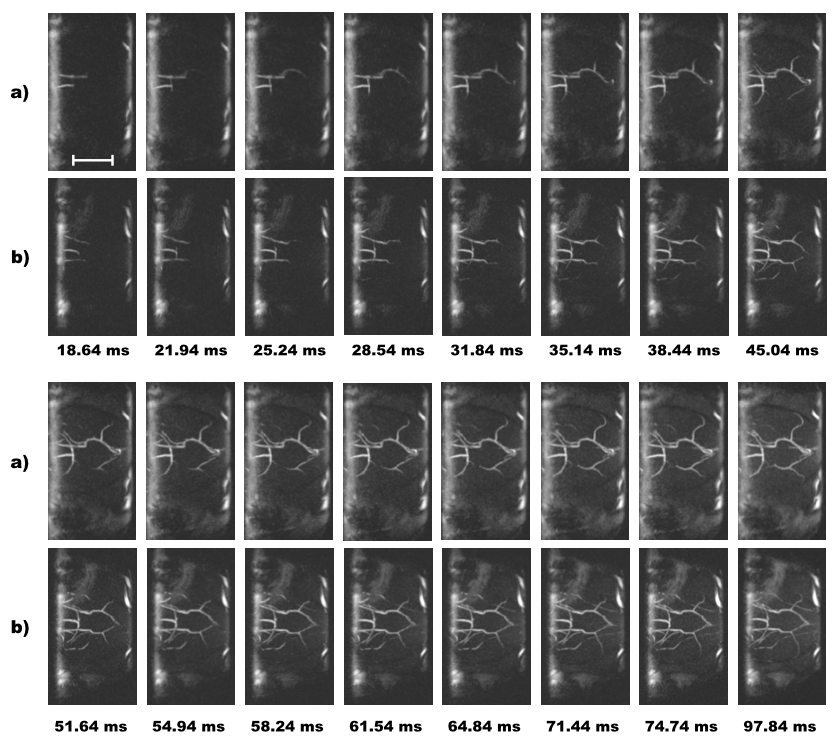
\includegraphics[scale=0.5]{./figure/chap3/ImFlowWillis.png}
\caption[Image d'ARM dynamique sur souris du polygone de Willis]{\label{fig:ImFlowWillis} Image MIP d'ARM dynamique acquises sur une souris saine (a) et pour une souris ayant subit une ligature des artères carotides (b). 16 images ont été extraites des 30 images cinés acquises.}
\line(1,0){400} \\ \end{figure}

\begin{figure}[H]
\centering \line(1,0){400} \\
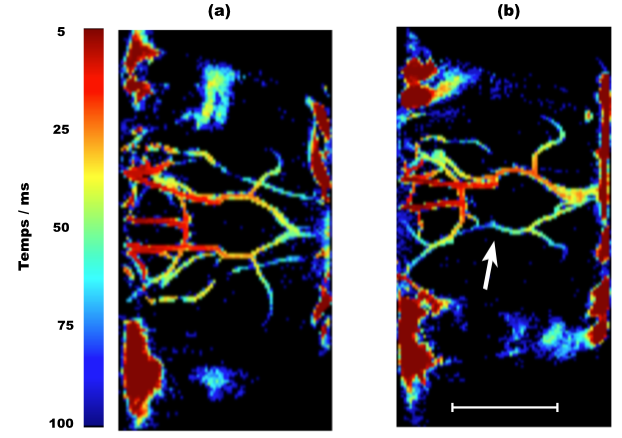
\includegraphics[scale=0.5]{./figure/chap3/ColorMapFlowWillis.png}
\caption[Image d'ARM dynamique sur souris du polygone de Willis]{\label{fig:ColorMapFlowWillis} Carte de couleur représentant la durée avant l'arrivée du sang dans une partie du polygone de Willis pour une souris saine (a) et une souris avec une artère carotide ligaturée (b).}
\line(1,0){400} \\ \end{figure}

Il n'est pas possible d'effectuer l'imagerie sur une plus large zone (par example des carotides au polygone). En effet, le contraste étant basé sur le principe du temps de vol, celui-ci sera saturé en arrivant à la fin du polygone. Une des solutions est d'augmenter le TR de la séquence mais nous obtiendrons une moins bonne visualisation dynamique de l'avancée du flux. De plus, la différence entre deux images consécutives sera plus importante ce qui limitera la taille du filtre temporel que l'on pourra utiliser. Enfin un dernier problème se pose puisqu'il faudrait augmenter le nombre d'images cinés à lire après la saturation du signal et donc que le signal statique aura repousser suffisamment pour encore diminuer le contraste que l'on pourrait espérer obtenir entre le cerveaux et les vaisseaux.

L'alternative employé a été de répéter la séquence 3 fois de suite en modifiant la position de la coupe puis à associer les images après leurs reconstructions en fonction de leurs positions (figure \ref{fig:FluxComplet}.a). On peut aussi reconstruire une carte de couleur mais cela demande à l'utilisateur d'indiquer à quel moment le flux d'une coupe entre dans la suivante. La figure \ref{fig:FluxComplet}.b est un example de représentation en carte de couleur utilisant de multiples coupes. On observe sur ces images des artéfacts au bord des coupes qui sont due à la mauvaise saturation du signal au bord de la sélection de coupe.

\begin{figure}[H]
\centering \line(1,0){400} \\
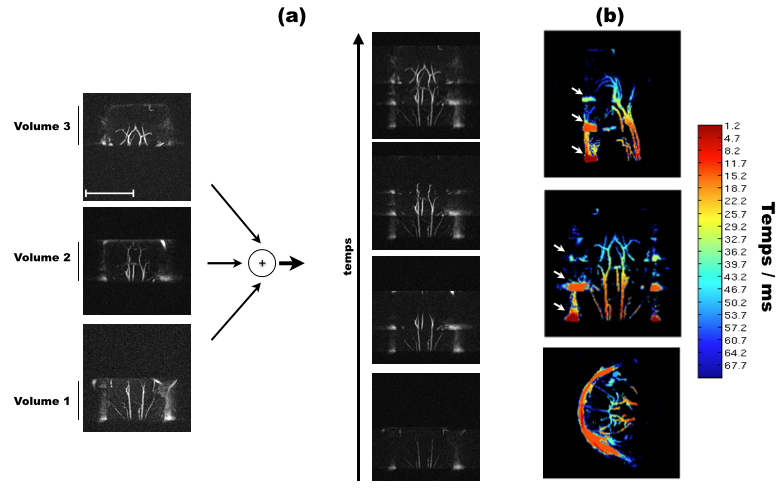
\includegraphics[scale=0.6]{./figure/chap3/FluxComplet.png}
\caption[Image d'ARM dynamique sur souris des carotides au polygone de Willis]{\label{fig:FluxComplet} Imagerie des carotides au polygone effectuée avec 3 acquisitions successives avec des coupes en 3 positions différentes. (a) L'association des images est effectuées après la reconstruction de chacune d'entre elles. (b) La carte de couleur représentant l'avancée des flux doit être synchronisé pour que l'arrivée d'une du sang dans la prochaine coupe débutent en même temps que le début de la prochaine.}
\line(1,0){400} \\ \end{figure}

\section{Discussion}

L'imagerie de flux chez la souris est un véritable défi du fait de la dimension des vaisseaux des paramètres physiologiques particuliers de la souris. De telles méthodes permettraient de mieux décrire le phénotype des modèles et suivre l'évolution des pathologies lors d'études longitudinales. Le développement de nouvelles méthodes d'imageries 4D de flux dynamique, offrant une résolution spatiale et temporelle élevée durant un temps d'acquisition raisonnable sont nécessaires pour accéder avec précision aux données fonctionnelles des flux.

Dans cette optique nous avons tout d'abord développé une séquence avec une trajectoire 3D radiale (PR) pour l'ARM anatomique. En effet, cette méthode est moins sensible aux artéfacts de flux et de mouvements que l'imagerie cartésienne ce qui permet d'obtenir des images anatomiques de la crosse aortique avec un signal très homogène malgré la respiration et les flux turbulent durant la phase systolique du coeur. 
De plus, la possibilité de sous-échantillonnage de cette méthode nous a permis d'obtenir des images ayant une qualité satisfaisante avec seulement 4000 projections correspondant à une diminution du temps d'acquisition supérieur à 14 par rapport au critère de Nyquist ainsi que de 10 par rapport à une séquence cartésienne standard permettant d'obtenir des images avec le même champ-de-vue. Dans le cas de l'utilisation d'une antenne surfacique il est possible de réduire avec la séquence cartésienne le nombre de pas de phase à recueillir dans l'une des directions, le facteur d'accélération de la séquence radiale est dans ce cas d'environ 4.
Le troisième avantage de l'imagerie radiale est l'utilisation d'une trajectoire pseudo-aléatoire. Cela permet une distribution approximativement uniforme des projections au cours du temps. Cette méthode peut être employé pour répartir efficacement les projections avec pour objectif de retirer les projections corrompues par les mouvements physiologiques. En effet il existe des approches utilisant les points centraux des projections pour extraire des informations sur la position de celles-ci au sein de la respiration. Il peut donc être possible de reconstruire à posteriori des images à différents moments de la phase de respiration, ou bien de reconstruire des images seulement grâce aux projections recueillies durant les phases de respiration avec peu de mouvement.
Grâce à ces différents points, l'imagerie radiale utilisant une trajectoire d'angle d'or peut être particulièrement efficace pour l'imagerie anatomique temps-de-vol, en particulier si les temps d'acquisition ont besoin d'être limité ou sur des régions anatomiques propice aux mouvements. 

Cette approche a ensuite été étendu à l'imagerie résolue dans le temps pour visualiser la progression des flux dans les vaisseaux avec une forte résolution temporelle de 3,3 ms, une forte résolution spatiale et surtout en un temps d'acquisition réduit par 5 par rapport à la méthode précédemment employée par Miraux et al.
L'optimisation de la séquence permet d'obtenir des temps de répétition inférieur à 3,5 ms qui sont nécessaire pour visualiser l'avancée des flux rapides dans les artères. Cela est aussi important pour permettre l'utilisation du filtre temporel qui est plus efficace lorsqu'il existe peu de différence entre les images adjacentes.
L'utilisation du filtre temporel a été rendu possible grâce à l'ajout du second angle d'or entre les trajectoires des images cinés. Celui-ci a pour effet de particulièrement bien répartir les projections entre celle-ci et permet une utilisation optimal de nombreuses formes de filtre temporel comme les filtres linéaires \cite{Barger:2002fk}, KWIC \cite{Song2004Dynamic-MRI-wit}, exponentielles etc. Cela est particulièrement important lorsque la dynamique des flux n'est pas connu ou potentiellement perturbé dans des modèles pathologiques où la résolution finale des images pourra être modulé pour obtenir des images avec une qualité adapté à la quantification de la vitesse des flux.

Plusieurs limitations sont cependant à noter concernant la méthode d'angiographie par temps-de-vol. En effet, pour la visualisation de flux lents, le sang sera saturé après avoir traversé une faible distance. Il est possible d'augmenter le temps de répétition de la séquence pour saturer le sang moins souvent cependant on obtiendra rapidement un faible contraste sur bruit entre le sang et les tissus environnants qui auront le temps de voir leur signal repousser après la saturation. L'autre possibilité est d'utiliser des coupes plus fines et de multiplier le nombre d'acquisition en déplaçant la position de la coupe. L'image disposera d'un peu moins de signal sur bruit car la signal sera accumulé moins de fois mais cela permettra de maintenir un bon contraste entre le sang et les tissus. Cependant cette  approche n'est pas adapté à l'imagerie avec des séquences radiales 3D car une grande partie de l'espace de Fourier échantillonné n'est pas nécessaire pour la reconstruction ce qui diminuera l'avantage en temps d'acquisition par rapport aux trajectoires cartésiennes.
Chez l'humain, cette limitation risque d'apparaitre car les flux sont plus lents par rapport à la distance anatomique parcourues et aux champs de vue étudiées. Une utilisation de la séquence avec une trajectoire radiale 3D est donc difficile. Cependant une approche utilisant des trajectoires de type "stack-of-stars" radiale permettrait de pouvoir obtenir des coupes fines en limitant le temps d'acquisition des séquences mais tout de même d'obtenir les avantages des séquences radiales selon les axes perpendiculaire au plan de coupe. 

Cette méthode a à plusieurs reprises fait ses preuves pour la quantification de flux chez le petit animal. Grâce à l'utilisation de trajectoire 3D radiales, celle-ci permet d'obtenir une visualisation encore plus précise de la dynamique des flux mais surtout devient applicable sur des cohortes grâce aux temps d'acquisitions particulièrement court et à la robustesse de la méthode. Des développements supplémentaires apparaissent nécessaires afin d'optimiser cette méthode pour une application chez l'humain (implantation d'une trajectoire "stack-of-stars", suppression ou correction des données obtenues lors du mouvement respiratoire) mais l'utilisation de méthodes d'accélérations conventionnelles permet d'envisager des temps d'acquisition du même ordre que chez le petit animal. Cela permettrait donc d'obtenir des informations en 4D sur la vitesse de flux avec une forte résolution spatiale et temporelle au minimum deux fois plus rapidement qu'avec les méthodes conventionnelles d'imagerie de phase.

%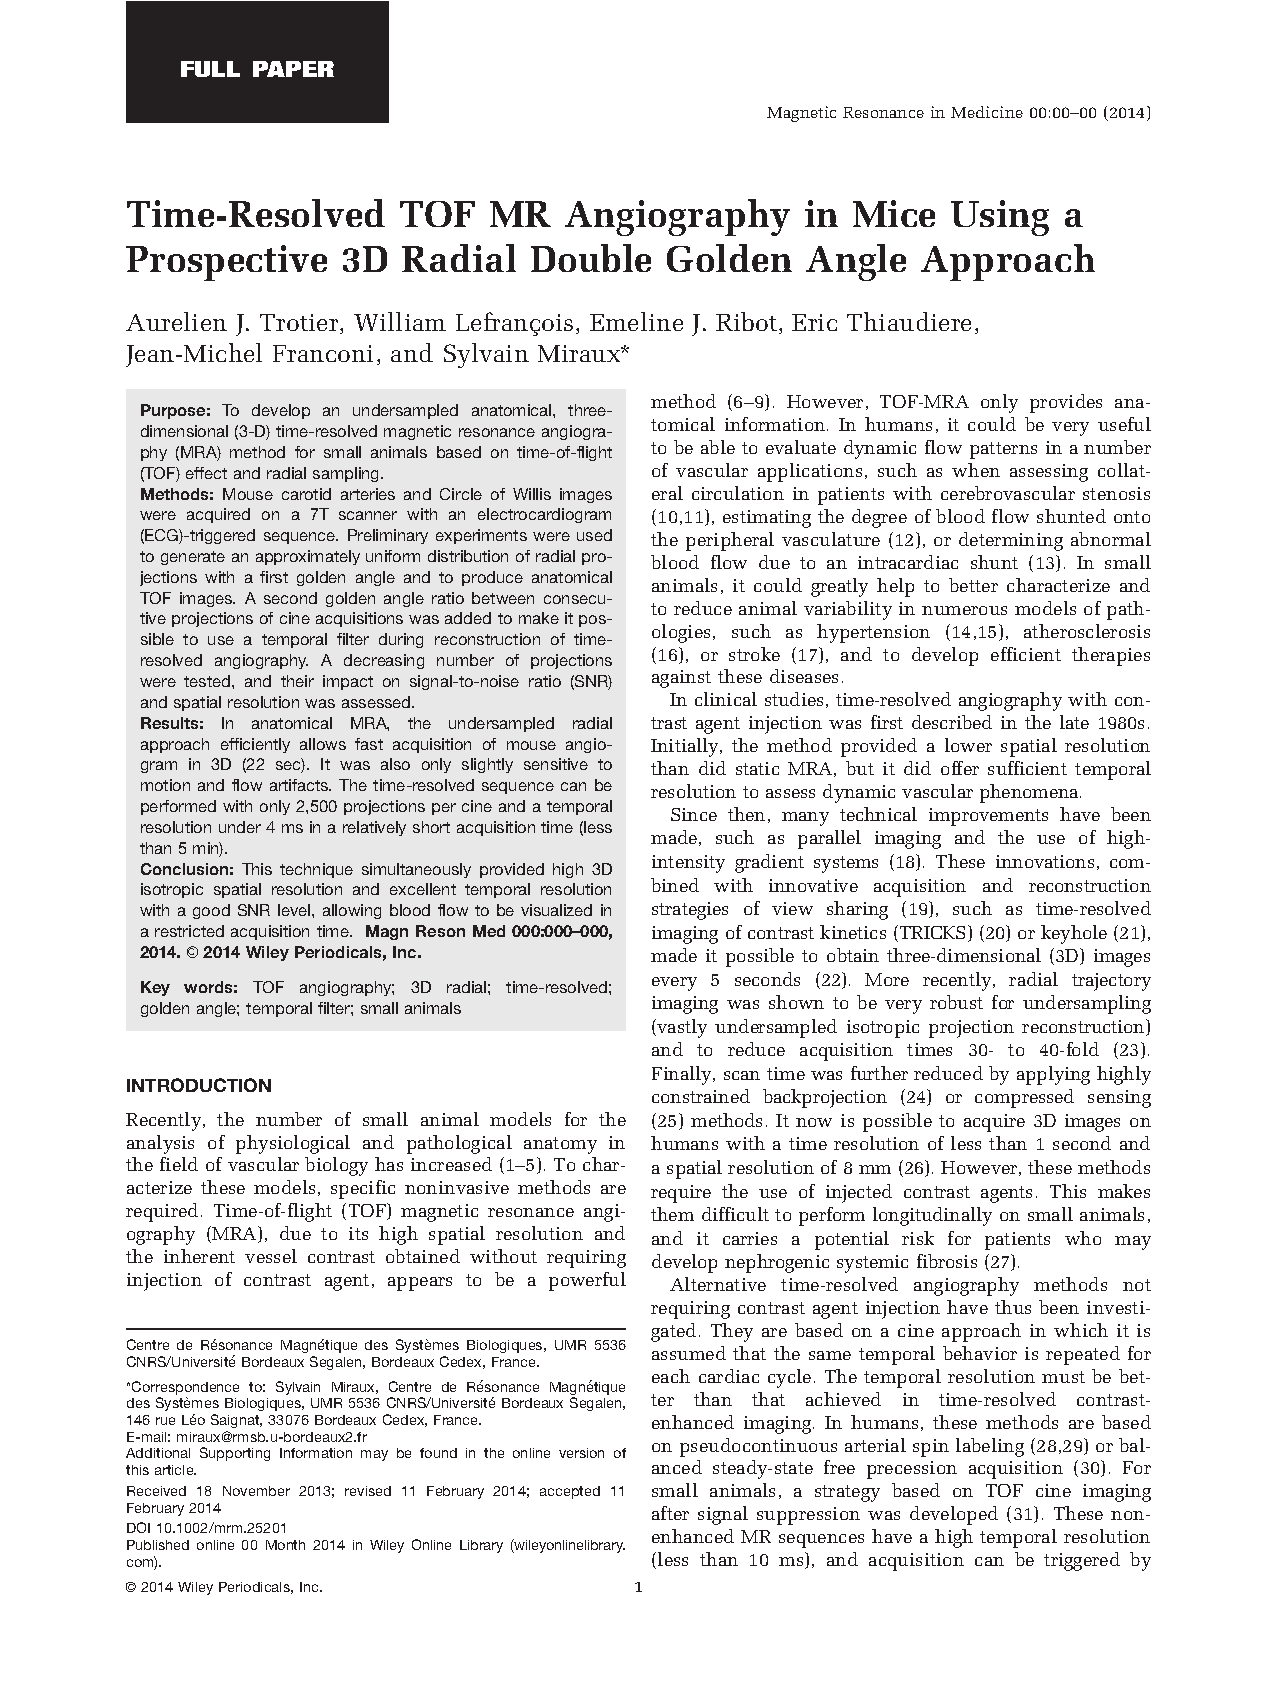
\includepdf[pages=1-11]{./figure/chap3/Papier1.pdf}